\documentclass[12pt,a4paper]{article}

% ---- Codificación y lengua ----
\usepackage[utf8]{inputenc}
\usepackage[T1]{fontenc}
\usepackage[provide=*,spanish]{babel}

% ---- Márgenes ----
\usepackage[top=2.5cm, bottom=2.5cm, left=3cm, right=2.5cm]{geometry}

% ---- Tipografía ----
\usepackage{lmodern}
\usepackage{microtype}

% ---- Matemáticas ----
\usepackage{amsmath}

% ---- Colores ----
\usepackage[dvipsnames,svgnames,table]{xcolor}
\definecolor{azulAS}{RGB}{30,90,160}
\definecolor{verdePos}{RGB}{46,125,50}
\definecolor{rojoNeg}{RGB}{183,28,28}
\definecolor{grisCelda}{RGB}{240,245,250}

% ---- Gráficos y figuras ----
\usepackage{graphicx}
\usepackage{float}
\usepackage{caption}
\captionsetup{font=small, labelfont=bf}

% ---- TikZ para diagramas ----
\usepackage{tikz}
\usetikzlibrary{shapes.geometric, arrows.meta, positioning, shapes}

% ---- Tablas ----
\usepackage{booktabs}
\usepackage{longtable}
\usepackage{array}
\usepackage{tabularx}
\usepackage{colortbl}

% ---- Código fuente ----
\usepackage{listings}
\lstset{
  basicstyle=\ttfamily\footnotesize,
  backgroundcolor=\color{grisCelda},
  frame=single,
  breaklines=true,
  captionpos=b,
  keywordstyle=\color{azulAS}\bfseries,
  commentstyle=\color{verdePos},
  stringstyle=\color{rojoNeg},
  language=Python,
  numbers=left,
  numberstyle=\tiny\color{gray},
  numbersep=5pt,
  showstringspaces=false,
  tabsize=2,
  extendedchars=true,
  inputencoding=utf8,
  literate=
    {á}{{\'a}}1 {é}{{\'e}}1 {í}{{\'i}}1 {ó}{{\'o}}1 {ú}{{\'u}}1
    {Á}{{\'A}}1 {É}{{\'E}}1 {Í}{{\'I}}1 {Ó}{{\'O}}1 {Ú}{{\'U}}1
    {ñ}{{\~n}}1 {Ñ}{{\~N}}1
    {ü}{{\"u}}1 {¿}{{?`}}1 {¡}{{!`}}1
}

% ---- Hipervínculos ----
\usepackage[colorlinks=true, linkcolor=azulAS, citecolor=verdePos,
            urlcolor=azulAS, bookmarks=true]{hyperref}

% ---- Encabezados ----
\usepackage{fancyhdr}
\setlength{\headheight}{14pt}
\pagestyle{fancy}
\fancyhf{}
\fancyhead[L]{\small El Observador Digital}
\fancyhead[R]{\small \thepage}
\renewcommand{\headrulewidth}{0.4pt}

\emergencystretch=3em

% ---- Espaciado ----
\usepackage{setspace}
\onehalfspacing

% ---- Secciones con color ----
\usepackage{titlesec}
\titleformat{\section}{\large\bfseries\color{azulAS}}{\thesection.}{0.5em}{}[\titlerule]
\titleformat{\subsection}{\normalsize\bfseries\color{azulAS}}{\thesubsection.}{0.5em}{}
\titleformat{\subsubsection}{\normalsize\itshape\color{azulAS}}{\thesubsubsection.}{0.5em}{}

% ---- Enumeraciones ----
\usepackage{enumitem}

\begin{document}

%---------------------------------------------------------------
% CARÁTULA
%---------------------------------------------------------------
\begin{titlepage}
  \thispagestyle{empty}
  \singlespacing
  \centering

  \vspace*{0.5cm}

  {\Large\bfseries Universidad Mayor de San Andrés}\\[0.3em]
  {\normalsize Facultad de Ciencias Puras y Naturales}\\[0.15em]
  {\normalsize Carrera de Informática}

  \vspace{0.5cm}

  
\includegraphics[width=2.8cm]{imagenes/Logo_Umsa.png}

  \vspace{0.6cm}

  {\color{azulAS}\rule{\linewidth}{1.5pt}}
  \vspace{0.35cm}

  {\LARGE\bfseries El Observador Digital}\\[0.35em]
  {\large Plataforma de análisis comparativo\\[0.15em]
   de medios bolivianos}

  \vspace{0.35cm}
  {\color{azulAS}\rule{\linewidth}{1.5pt}}

  \vspace{0.7cm}

  {\large Maximiliano Gómez Mallo}\\[0.15em]
  {\normalsize 14480221}

  \vspace{0.7cm}

  \begin{tabular}{ll}
    \textbf{Materia:}  & Minería de Datos \\[0.25em]
    \textbf{Docente:}  & Menfy Morales Rios \\[0.25em]
    \textbf{Fecha:}    & La Paz, Bolivia --- Mayo 2026 \\
  \end{tabular}

\end{titlepage}

\tableofcontents
\newpage

% ============================================================
\section{Resumen Ejecutivo}
% ============================================================

\textbf{El Observador Digital} es una plataforma automática de monitoreo y análisis comparativo de medios de comunicación bolivianos. El sistema vigila seis portales de noticias --- Red Uno, El Deber, Brújula Digital, Los Tiempos, Erbol y La Razón --- recolectando artículos nuevos \textbf{una vez al día} y procesándolos con técnicas de inteligencia artificial local y en la nube.

El flujo de trabajo central es el siguiente: los artículos recién descargados se convierten en vectores numéricos mediante un modelo de lenguaje local (\textit{MiniLM-L12-v2}), se calcula la similitud entre ellos y se agrupan automáticamente aquellos que tratan el mismo evento noticioso. Solo se forma un evento si al menos \textbf{dos medios distintos} cubren el mismo hecho --- esto garantiza que el sistema detecta únicamente noticias con cobertura cruzada real, descartando artículos aislados. Posteriormente, la API de Gemini analiza el tono editorial de cada artículo y detecta diferencias de encuadre entre los distintos medios que cubren el mismo hecho.

Los resultados son accesibles a través de una interfaz web con estética de periódico clásico: portada con tarjetas visuales (incluida la imagen de portada de cada evento), cronología de eventos con gráfico de dispersión por sesgo e importancia, y visualización detallada de sesgos editoriales. Adicionalmente, el sistema ofrece un asistente de inteligencia artificial conversacional flotante que responde preguntas sobre los datos monitoreados en lenguaje natural y devuelve tarjetas con los eventos o artículos más relevantes para cada consulta.

La plataforma corre en un servidor VPS con costes de infraestructura mínimos: el modelo de \textit{embeddings} funciona en CPU sin costo alguno, y la API de Gemini se usa en el nivel gratuito.

% ============================================================
\section{Motivación}
% ============================================================

Bolivia tiene un ecosistema mediático marcadamente fragmentado. Los principales diarios y portales de noticias se concentran en tres ciudades --- Santa Cruz de la Sierra, Cochabamba y La Paz --- y cada uno responde a una línea editorial propia, condicionada por factores regionales, económicos y políticos. Este fenómeno es conocido en el ámbito del periodismo como \textit{sesgo editorial}: la tendencia de un medio a presentar un mismo hecho desde un encuadre particular, seleccionando ciertos datos, omitiendo otros y eligiendo un vocabulario con carga valorativa.

Un ejemplo cotidiano: una manifestación en La Paz puede aparecer en un portal paceño como ``protesta ciudadana legítima'' y en un diario cruceño como ``bloqueo que afecta la economía''. Ambos describen el mismo evento; ninguno miente; pero la percepción que transmiten al lector es radicalmente distinta.

Monitorear manualmente estos sesgos es inviable. Un analista tendría que leer decenas de artículos al día de múltiples portales, identificar cuáles tratan el mismo tema, compararlos y registrar las diferencias. El tiempo necesario para esa tarea supera con creces los recursos de cualquier investigador individual.

\textbf{El Observador Digital} automatiza ese proceso completo. En lugar de requerir intervención humana para agrupar artículos o detectar diferencias editoriales, el sistema:

\begin{itemize}[nosep]
  \item Descarga artículos de seis portales de forma continua y estructurada.
  \item Identifica automáticamente qué artículos de distintos medios hablan del mismo evento, sin necesidad de que compartan palabras clave exactas.
  \item Cuantifica y visualiza las diferencias de encuadre entre medios para el mismo evento.
  \item Proporciona una interfaz de consulta en lenguaje natural para que cualquier usuario pueda explorar los datos.
\end{itemize}

El objetivo no es juzgar qué medio es más o menos confiable, sino ofrecer una herramienta transparente que permita al lector ver el panorama completo de cómo se está cubriendo un tema en Bolivia.

% ============================================================
\section{Arquitectura General}
% ============================================================

El sistema está organizado en cuatro capas funcionales que operan como un \textit{pipeline} secuencial. La Figura~\ref{fig:arquitectura} muestra el flujo de datos desde la recolección hasta la presentación.

\begin{figure}[h]
\centering
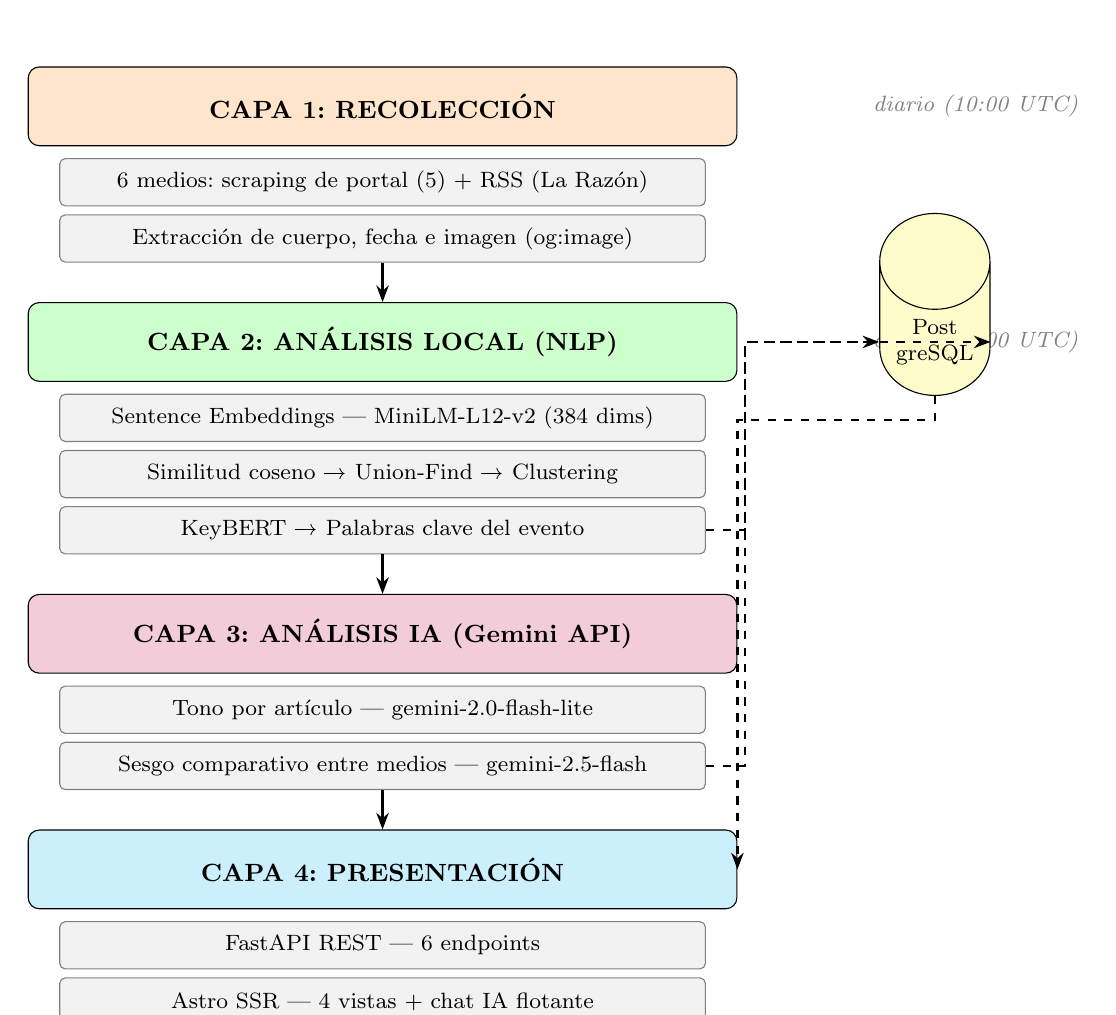
\begin{tikzpicture}[
  node distance=0.7cm,
  box/.style={
    rectangle, rounded corners=4pt,
    draw=black, fill=blue!10,
    minimum width=9cm, minimum height=1cm,
    align=center, font=\small\bfseries
  },
  subbox/.style={
    rectangle, rounded corners=2pt,
    draw=gray, fill=gray!10,
    minimum width=8.2cm, minimum height=0.6cm,
    align=center, font=\footnotesize
  },
  arrow/.style={-{Stealth[length=6pt]}, thick},
  sidelabel/.style={font=\footnotesize\itshape, text=gray}
]

% Capa 1
\node[box, fill=orange!20] (L1) {CAPA 1: RECOLECCIÓN};
\node[subbox, below=0.15cm of L1] (L1a) {6 medios: scraping de portal (5) + RSS (La Razón)};
\node[subbox, below=0.1cm of L1a] (L1b) {Extracción de cuerpo, fecha e imagen (og:image)};

% Capa 2
\node[box, fill=green!20, below=0.5cm of L1b] (L2) {CAPA 2: ANÁLISIS LOCAL (NLP)};
\node[subbox, below=0.15cm of L2] (L2a) {Sentence Embeddings --- MiniLM-L12-v2 (384 dims)};
\node[subbox, below=0.1cm of L2a] (L2b) {Similitud coseno → Union-Find → Clustering};
\node[subbox, below=0.1cm of L2b] (L2c) {KeyBERT → Palabras clave del evento};

% Capa 3
\node[box, fill=purple!20, below=0.5cm of L2c] (L3) {CAPA 3: ANÁLISIS IA (Gemini API)};
\node[subbox, below=0.15cm of L3] (L3a) {Tono por artículo --- gemini-2.0-flash-lite};
\node[subbox, below=0.1cm of L3a] (L3b) {Sesgo comparativo entre medios --- gemini-2.5-flash};

% Capa 4
\node[box, fill=cyan!20, below=0.5cm of L3b] (L4) {CAPA 4: PRESENTACIÓN};
\node[subbox, below=0.15cm of L4] (L4a) {FastAPI REST --- 6 endpoints};
\node[subbox, below=0.1cm of L4a] (L4b) {Astro SSR --- 4 vistas + chat IA flotante};

% Scheduler (lateral)
\node[sidelabel, right=0.4cm of L1, xshift=1.2cm] (S1) {diario (10:00 UTC)};
\node[sidelabel, right=0.4cm of L2, xshift=1.2cm] (S2) {diario (11:00 UTC)};

% Flechas principales
\draw[arrow] (L1b) -- (L2);
\draw[arrow] (L2c) -- (L3);
\draw[arrow] (L3b) -- (L4);

% Base de datos lateral
\node[cylinder, shape border rotate=90, draw=black, fill=yellow!20,
      minimum height=1.2cm, minimum width=1.4cm,
      right=1.8cm of L2, font=\footnotesize, align=center] (DB)
      {Post\\greSQL};

\draw[arrow, dashed] (L2c.east) -- ++(0.5,0) |- (DB.west);
\draw[arrow, dashed] (L3b.east) -- ++(0.5,0) |- (DB.east);
\draw[arrow, dashed] (DB.south) -- ++(0,-0.3) -| (L4.east);

\end{tikzpicture}
\caption{Pipeline de cuatro capas del sistema El Observador Digital.}
\label{fig:arquitectura}
\end{figure}

El \textbf{programador de tareas} (\textit{APScheduler}) coordina dos ciclos diarios: recolección a las 10:00 UTC y análisis a las 11:00 UTC. El ciclo de recolección descarga artículos nuevos y sus imágenes de portada; el ciclo de análisis agrupa los artículos en eventos y ejecuta el análisis editorial con Gemini. Ambos ciclos son independientes: el análisis siempre trabaja sobre los artículos ya almacenados en la base de datos.

% ============================================================
\section{Recolección de Datos mediante Web Scraping}
% ============================================================

El web scraping es la técnica central de este proyecto. Dado que los medios bolivianos no ofrecen APIs públicas ni feeds confiables, el sistema extrae información directamente del HTML de sus portales de forma automatizada. Esta sección describe en detalle la arquitectura, las estrategias por medio, el manejo de errores HTTP y los algoritmos de extracción de contenido.

\subsection{El problema del RSS en medios bolivianos}

La sindicación RSS es el mecanismo estándar que los portales exponen para que agregadores reciban contenido nuevo. En teoría, basta con suscribirse al feed de cada medio. En la práctica boliviana ese supuesto falla por dos razones:

\begin{itemize}[nosep]
  \item Varios portales relevantes no ofrecen feed RSS o lo tienen deshabilitado. Este es un problema común en países donde el mantenimiento técnico de los portales de noticias es esporádico y los equipos de desarrollo son reducidos.
  \item Los feeds que sí existen se actualizan con un retraso de dos a tres semanas: el equipo publica primero en la web y el RSS se actualiza de forma manual o nunca.
\end{itemize}

La solución adoptada es un enfoque \textbf{híbrido}: scraping directo del portal para cinco medios (Red Uno, El Deber, Brújula Digital, Los Tiempos, Erbol) y RSS únicamente para La Razón, cuyo sitio es una \textit{Single Page Application} (SPA) renderizada con JavaScript que hace imposible el scraping tradicional del DOM.

\subsection{Arquitectura del pipeline de scraping}

El proceso se divide en dos etapas secuenciales dentro del ciclo diario de recolección:

\begin{figure}[H]
\centering
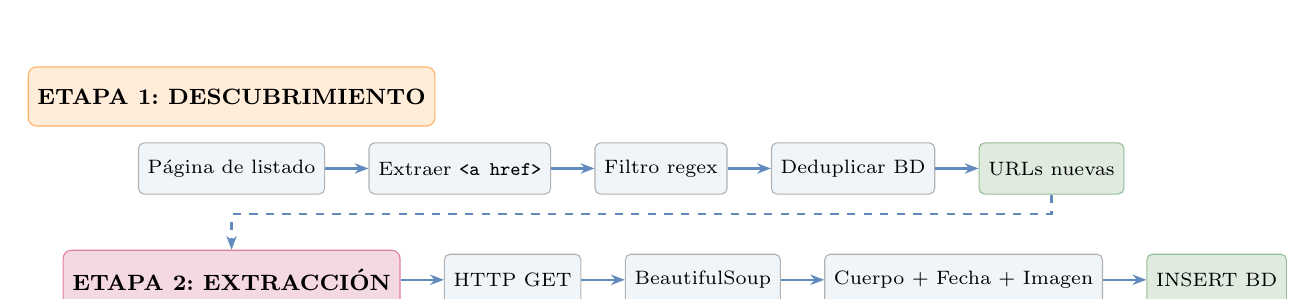
\begin{tikzpicture}[
  node distance=0.45cm and 0.55cm,
  box/.style={rectangle, rounded corners=3pt, draw=azulAS, fill=azulAS!10,
              minimum height=0.75cm, align=center, font=\footnotesize\bfseries},
  sbox/.style={rectangle, rounded corners=2pt, draw=gray!60, fill=grisCelda,
               minimum height=0.65cm, align=center, font=\scriptsize},
  arr/.style={-{Stealth[length=5pt]}, thick, color=azulAS!70},
  stage/.style={rectangle, draw=azulAS, dashed, rounded corners=4pt,
                inner sep=6pt, fill=azulAS!3}
]

% Etapa 1
\node[box, fill=orange!15, draw=orange!60] (E1) {ETAPA 1: DESCUBRIMIENTO};
\node[sbox, below=0.2cm of E1] (s1) {Página de listado};
\node[sbox, right=of s1] (s2) {Extraer \texttt{<a href>}};
\node[sbox, right=of s2] (s3) {Filtro regex};
\node[sbox, right=of s3] (s4) {Deduplicar BD};
\node[sbox, right=of s4, fill=verdePos!15, draw=verdePos!50] (s5) {URLs nuevas};

\draw[arr] (s1) -- (s2);
\draw[arr] (s2) -- (s3);
\draw[arr] (s3) -- (s4);
\draw[arr] (s4) -- (s5);

% Etapa 2
\node[box, fill=purple!15, draw=purple!50, below=0.7cm of s1] (E2) {ETAPA 2: EXTRACCIÓN};
\node[sbox, right=of E2] (t1) {HTTP GET};
\node[sbox, right=of t1] (t2) {BeautifulSoup};
\node[sbox, right=of t2] (t3) {Cuerpo + Fecha + Imagen};
\node[sbox, right=of t3, fill=verdePos!15, draw=verdePos!50] (t4) {INSERT BD};

\draw[arr] (E2) -- (t1);
\draw[arr] (t1) -- (t2);
\draw[arr] (t2) -- (t3);
\draw[arr] (t3) -- (t4);

% Conexión entre etapas
\draw[arr, dashed] (s5.south) -- ++(0,-0.25) -| (E2.north);

\end{tikzpicture}
\caption{Pipeline de scraping en dos etapas: descubrimiento de URLs y extracción de contenido.}
\label{fig:scraping_pipeline}
\end{figure}

La \textbf{Etapa 1} (descubrimiento) descarga la portada de cada medio, extrae todos los hipervínculos y aplica un filtro por expresión regular para quedarse solo con URLs de artículos. La \textbf{Etapa 2} (extracción) visita cada URL nueva y extrae el cuerpo textual, la fecha de publicación y la imagen de portada.

\subsection{Configuración por medio: patrones de URL}

Cada portal tiene una estructura de URLs distinta. La Tabla~\ref{tab:scraping_medios} resume la estrategia y el patrón regex usado para cada medio.

\begin{table}[H]
\centering
\caption{Estrategia de scraping y patrón de URL por medio}
\label{tab:scraping_medios}
\begin{tabular}{@{}p{3cm}p{2cm}p{5.5cm}p{2.5cm}@{}}
\toprule
\rowcolor{azulAS!15}
\textbf{Medio} & \textbf{Estrategia} & \textbf{Patrón regex} & \textbf{Característica} \\
\midrule
Red Uno & Portal & \texttt{/(noticias|..)/\textbackslash S+\textbackslash d\{6,\}} & $\geq$6 dígitos en path \\
\rowcolor{grisCelda}
El Deber & Portal & \texttt{\^{}/[a-z-]+/[a-z0-9-]\{10,\}\_} & Slug con \texttt{\_} al final \\
Brújula Digital & Portal & \texttt{\^{}/[a-z-]+/[a-z0-9-]\{10,\}} & Slug $\geq$10 caracteres \\
\rowcolor{grisCelda}
Los Tiempos & Portal & \texttt{/\textbackslash d\{8\}/} & 8 dígitos consecutivos \\
Erbol & Portal & \texttt{\^{}/[\^{}/\textbackslash s]+/[\^{}/\textbackslash s]\{10,\}\$} & Acepta chars URL-encoded \\
\rowcolor{grisCelda}
La Razón & RSS & Feed XML (feedparser) & SPA React, sin DOM estático \\
\bottomrule
\end{tabular}
\end{table}

El diccionario \texttt{CONFIGS} en \texttt{portal.py} centraliza esta configuración. Cada entrada define la URL de listado, la URL base para normalizar href relativos, el patrón regex de artículo y una lista de fragmentos a excluir (páginas de tags, autores, búsquedas):

\begin{lstlisting}[language=Python, caption=Configuración de scraping por medio (portal.py)]
CONFIGS = {
    "El Deber": {
        "listing_url": "https://eldeber.com.bo",
        "base_url":    "https://eldeber.com.bo",
        "url_pattern": r"^/[a-z\-]+/[a-z0-9\-]{10,}_",
        "exclude_fragments": ["/tag/", "/autor/", "/seccion/"],
    },
    "Los Tiempos": {
        "listing_url": "https://www.lostiempos.com",
        "base_url":    "https://www.lostiempos.com",
        "url_pattern": r"/\d{8}/",
        "exclude_fragments": [],
    },
    # ... Red Uno, Erbol, Brujula Digital
}
\end{lstlisting}

\subsection{HTTP robusto: reintentos con backoff exponencial}

Los portales bolivianos presentan inestabilidad frecuente: Brújula Digital y Erbol retornan HTTP 500 en una fracción de artículos, y Red Uno ocasionalmente limita la velocidad de acceso. La función \texttt{\_fetch()} implementa reintentos con \textbf{espera exponencial} para manejar estos fallos de forma transparente:

\begin{lstlisting}[language=Python, caption=Función \_fetch con reintentos y backoff exponencial (portal.py)]
HEADERS = {
    "User-Agent": "Mozilla/5.0 (Windows NT 10.0; Win64; x64) "
                  "AppleWebKit/537.36 Chrome/124.0 Safari/537.36",
    "Accept": "text/html,application/xhtml+xml,*/*;q=0.8",
    "Accept-Language": "es-ES,es;q=0.9",
}

def _fetch(url, reintentos=3):
    for i in range(reintentos):
        try:
            r = requests.get(url, headers=HEADERS, timeout=15)
            if r.status_code == 200:
                return r.text
            logger.warning(f"HTTP {r.status_code} en {url}")
        except Exception as e:
            logger.warning(f"Intento {i+1} fallido para {url}: {e}")
        if i < reintentos - 1:
            time.sleep(2 ** i)  # 1s, 2s entre intentos
    return None
\end{lstlisting}

Aspectos relevantes de la implementación:

\begin{itemize}[nosep]
  \item \textbf{User-Agent realista}: simula un navegador Chrome para evitar bloqueos por bots. Varios portales bolivianos rechazan peticiones con \texttt{python-requests} como User-Agent.
  \item \textbf{Timeout de 15 segundos}: evita que una conexión colgada bloquee el ciclo completo de scraping.
  \item \textbf{Backoff exponencial}: espera $2^0=1$ segundo tras el primer fallo y $2^1=2$ segundos tras el segundo, reduciendo la carga sobre el servidor en momentos de alta demanda.
  \item \textbf{Fallo silencioso}: si los 3 intentos fallan, retorna \texttt{None} y el artículo queda pendiente para el siguiente ciclo diario.
\end{itemize}

Una vez obtenido el HTML, la extracción de URLs de artículos filtra en dos niveles: primero aplica el patrón regex del medio, luego verifica que ningún fragmento excluido esté presente en el path. Los títulos con menos de 10 caracteres (links de iconos o imágenes sin texto) también se descartan.

Para mantener el volumen de artículos manejable y no sobrecargar el análisis de Gemini, se impone un \textbf{límite de 20 artículos nuevos por medio por ciclo} (\texttt{MAX\_POR\_MEDIO = 20}). Si una portada contiene más URLs nuevas, se descartan las excedentes. En la práctica, la deduplicación por URL hace que la mayoría de ciclos encuentren muchos menos de 20 artículos nuevos por medio, ya que los artículos del día anterior ya están almacenados.

\subsection{Extracción del cuerpo y la fecha del artículo}

La heterogeneidad de los portales bolivianos --- algunos usan WordPress, otros sistemas propietarios, otros frameworks modernos --- obliga a una estrategia de extracción tolerante a la variación de estructura HTML.

\subsubsection{Selectores CSS en cascada}

\texttt{article.py} define una lista ordenada de 8 selectores CSS que se prueban secuencialmente. Se usa el primero que devuelva un bloque de texto con al menos 200 caracteres:

\begin{table}[H]
\centering
\caption{Selectores CSS en orden de prioridad para extracción del cuerpo}
\begin{tabular}{@{}clp{7cm}@{}}
\toprule
\rowcolor{azulAS!15}
\textbf{\#} & \textbf{Selector} & \textbf{Justificación} \\
\midrule
1 & \texttt{article} & Elemento HTML5 semántico; estándar en CMS modernos \\
\rowcolor{grisCelda}
2 & \texttt{[class*='article-body']} & Clase más usada en portales de noticias personalizados \\
3 & \texttt{[class*='article\_body']} & Variante con guión bajo \\
\rowcolor{grisCelda}
4 & \texttt{[class*='content-body']} & Patrón alternativo \\
5 & \texttt{[class*='nota-body']} & Terminología de medios hispanohablantes \\
\rowcolor{grisCelda}
6 & \texttt{[class*='cuerpo']} & Término en español, común en portales bolivianos \\
7 & \texttt{.entry-content} & Clase estándar de WordPress \\
\rowcolor{grisCelda}
8 & \texttt{main} & Fallback final: elemento HTML5 \texttt{main} \\
\bottomrule
\end{tabular}
\end{table}

Antes de aplicar los selectores, se elimina el ``ruido'' del HTML: scripts, estilos, navegación, pie de página, sidebars y elementos publicitarios. Esto garantiza que el texto extraído sea solo el contenido editorial:

\begin{lstlisting}[language=Python, caption=Extracción robusta del cuerpo (article.py)]
SELECTORES = ["article", "[class*='article-body']",
              "[class*='article_body']", "[class*='content-body']",
              "[class*='nota-body']",  "[class*='cuerpo']",
              ".entry-content", "main"]

RUIDO = ["script", "style", "nav", "footer", "aside", "[class*='ad']"]

soup = BeautifulSoup(r.text, "lxml")

for selector in RUIDO:          # eliminar elementos no editoriales
    for tag in soup.select(selector):
        tag.decompose()

cuerpo = None
for selector in SELECTORES:     # probar selectores en cascada
    elemento = soup.select_one(selector)
    if elemento:
        texto = elemento.get_text(separator=" ", strip=True)
        if len(texto) >= 200:   # umbral de contenido minimo
            cuerpo = texto
            break
\end{lstlisting}

\subsubsection{Extracción de la fecha de publicación}

La fecha de publicación se extrae con tres métodos en orden de fiabilidad decreciente:

\begin{lstlisting}[language=Python, caption=Extracción de fecha en tres niveles de prioridad (article.py)]
def _extraer_fecha(soup):
    # 1. OpenGraph: mas estandarizado
    meta = soup.find("meta", property="article:published_time")
    if meta and meta.get("content"):
        f = _parse_fecha(meta["content"])
        if f: return f

    # 2. JSON-LD: datos estructurados embebidos
    for script in soup.find_all("script", type="application/ld+json"):
        try:
            data = json.loads(script.string or "")
            if isinstance(data, list): data = data[0]
            fecha_str = data.get("datePublished") or data.get("dateCreated")
            if fecha_str:
                f = _parse_fecha(fecha_str)
                if f: return f
        except Exception: pass

    # 3. <time datetime>: fallback HTML5
    time_tag = soup.find("time", attrs={"datetime": True})
    if time_tag:
        return _parse_fecha(time_tag["datetime"])
    return None
\end{lstlisting}

\subsection{Extracción de la imagen de portada (og:image)}

Los portales de noticias modernos publican una imagen destacada para cada artículo con el fin de que se muestre correctamente al compartir en redes sociales. Esta imagen se declara en el encabezado HTML como metadato \textbf{Open Graph} (\texttt{og:image}), un estándar ampliamente adoptado por Facebook, Twitter y WhatsApp.

\textbf{El Observador Digital} aprovecha este metadato para mostrar la imagen de portada de cada evento sin necesidad de alojar imágenes propias: simplemente se lee la URL que el propio portal ya declaró y se presenta en la interfaz.

\begin{lstlisting}[language=Python, caption=Extracción de imagen og:image (article.py)]
def _extraer_imagen(soup, base_url):
    """Retorna la URL absoluta de og:image, o None si no existe."""
    og = (soup.find("meta", property="og:image")
          or soup.find("meta", attrs={"name": "og:image"}))
    if not og:
        return None
    url = (og.get("content") or "").strip()
    if not url:
        return None
    # Convertir URL relativa a absoluta si es necesario
    if url.startswith("//"):
        return "https:" + url
    if url.startswith("/"):
        return base_url.rstrip("/") + url
    return url
\end{lstlisting}

La URL obtenida se almacena en la columna \texttt{imagen\_url} de la tabla \texttt{articulos} (añadida mediante una migración de Alembic). Cuando la API devuelve un evento, selecciona la primera imagen no nula entre sus artículos y la expone como \texttt{imagen\_url} del evento. En el frontend, si la imagen no carga (error HTTP, URL expirada), el componente muestra una franja de color de la categoría del evento como alternativa visual.

\subsection{Filtros de calidad}

Antes de insertar un artículo en la base de datos se aplican cuatro filtros que garantizan la integridad del corpus:

\begin{itemize}[nosep]
  \item \textbf{Deduplicación por URL}: la tabla tiene una restricción \texttt{UNIQUE} sobre la columna \texttt{url}; si ya existe, la inserción se omite sin error.
  \item \textbf{Título mínimo}: el título debe tener al menos 10 caracteres (elimina links de iconos o imágenes sin texto).
  \item \textbf{Cuerpo mínimo}: el cuerpo debe superar los 200 caracteres (descarta artículos de solo imagen, video o galería sin texto editorial).
  \item \textbf{Antigüedad máxima --- 7 días}: en la Etapa 2 (post-extracción de cuerpo), si la fecha del artículo supera los 7 días se elimina de la base de datos. Este filtro se aplica \textit{después} de extraer el cuerpo porque los portales no exponen la fecha hasta visitar el artículo individualmente. Los artículos sin fecha parseable se conservan por precaución. El feed RSS de La Razón aplica el mismo límite de 7 días al descubrir entradas.
  \item \textbf{Links muertos}: artículos que tras el scraping quedan sin cuerpo \textit{y} sin fecha (respuesta 404, página en blanco, error del portal) se eliminan de la base de datos automáticamente.
\end{itemize}

\subsection{Orquestación y ejecución periódica}

La función \texttt{correr\_scraping()} en \texttt{app/scraper/\_\_init\_\_.py} orquesta el pipeline completo en dos fases:

\begin{lstlisting}[language=Python, caption=Función de orquestación del scraping (\_\_init\_\_.py)]
def correr_scraping(db):
    stats = {"nuevos": 0, "cuerpos": 0, "errores": 0}
    medios = db.query(Medio).filter(Medio.activo == True).all()

    # Fase 1: descubrir nuevas URLs por medio
    for medio in medios:
        if medio.nombre in PORTAL_CONFIGS:
            stats["nuevos"] += scrape_portal(medio, db)  # scraping HTML
        else:
            stats["nuevos"] += fetch_feed(medio, db)     # RSS feedparser

    # Fase 2: extraer cuerpo, fecha e imagen de articulos sin completar
    sin_cuerpo = db.query(Articulo).filter(Articulo.cuerpo == None).all()
    for articulo in sin_cuerpo:
        resultado = scrape_articulo(articulo.url)
        if resultado["cuerpo"]:
            articulo.cuerpo = resultado["cuerpo"]
            stats["cuerpos"] += 1
        if resultado["fecha_publicacion"] and articulo.fecha_publicacion is None:
            articulo.fecha_publicacion = resultado["fecha_publicacion"]
        if resultado.get("imagen_url") and articulo.imagen_url is None:
            articulo.imagen_url = resultado["imagen_url"]

    db.commit()
    logger.info(f"Scraping completo: {stats}")
    return stats
\end{lstlisting}

Esta función es invocada por \textbf{APScheduler} con un disparador \textit{cron} a las 10:00 UTC cada día. La separación en dos fases es intencional: si un artículo nuevo se descubre en la Fase 1 pero falla la extracción (timeout, error HTTP), queda registrado en la BD con \texttt{cuerpo = NULL} y será reintentado en el siguiente ciclo diario.

\subsection{Manejo de zonas horarias}

Los portales bolivianos publican las fechas en hora local (UTC-4, sin horario de verano). La base de datos almacena estas fechas \textit{sin información de zona horaria} (\textit{naive datetime}) tal como vienen. La API REST aplica el sufijo adecuado al serializar:

\begin{itemize}[nosep]
  \item \texttt{fecha\_publicacion}: se añade el sufijo \texttt{-04:00} (hora boliviana).
  \item \textit{Timestamps} del sistema (fecha de scraping, detección de eventos): se añade \texttt{Z} (UTC).
\end{itemize}

% ============================================================
\section{Agrupación de Eventos con IA Local}
% ============================================================

\subsection{Representación vectorial de artículos (\textit{embeddings})}

El primer desafío para agrupar artículos es representarlos de una forma que la computadora pueda comparar. El texto en crudo no es directamente comparable: dos artículos sobre la misma huelga pueden no compartir ninguna palabra si uno usa ``paro'' y el otro ``huelga''.

La solución son los \textbf{embeddings semánticos}: una técnica que convierte cualquier texto en una lista de 384 números reales. La metáfora más útil es pensar en esos números como \textit{coordenadas GPS del significado}: textos sobre temas similares terminan cerca en ese espacio de 384 dimensiones, aunque usen vocabulario distinto.

El modelo utilizado es \textbf{MiniLM-L12-v2}, parte de la familia \textit{sentence-transformers}. Ocupa aproximadamente 120 MB, se descarga una sola vez y funciona íntegramente en CPU sin necesidad de GPU ni de llamadas a APIs externas. El coste computacional por artículo es de decenas de milisegundos.

\begin{lstlisting}[language=Python, caption=Generación de embeddings con sentence-transformers]
from sentence_transformers import SentenceTransformer

model = SentenceTransformer(
    "sentence-transformers/paraphrase-multilingual-MiniLM-L12-v2"
)

# texto = titulo + primeros 512 tokens del cuerpo
vector = model.encode(texto)  # -> array de 384 floats
\end{lstlisting}

\subsection{Similitud coseno}

Una vez que cada artículo tiene su vector, el siguiente paso es medir qué tan ``parecidos'' son dos artículos. La métrica usada es la \textbf{similitud coseno}:

\begin{equation}
  \cos(\theta) = \frac{\mathbf{A} \cdot \mathbf{B}}{|\mathbf{A}|\,|\mathbf{B}|} = \frac{\sum_{i=1}^{n} A_i B_i}{\sqrt{\sum_{i=1}^{n} A_i^2}\;\sqrt{\sum_{i=1}^{n} B_i^2}}
\end{equation}

Esta fórmula calcula el coseno del ángulo entre dos vectores. Su rango es de $-1$ a $1$; en la práctica, para vectores de texto generados por modelos modernos el rango efectivo es de $0$ a $1$:

\begin{itemize}[nosep]
  \item $1.0$: artículos idénticos en significado.
  \item $0.65$--$0.85$: artículos sobre el mismo evento con redacción diferente.
  \item $< 0.4$: artículos sobre temas no relacionados.
\end{itemize}

El umbral elegido para declarar que dos artículos pertenecen al mismo evento es $\mathbf{0.65}$. Este valor se determinó empíricamente: con $0.75$ se perdían artículos de distintos medios que cubrían el mismo hecho con vocabulario muy diferente; con $0.65$ se capturan esos casos sin agrupar artículos no relacionados.

\subsection{Algoritmo Union-Find para clustering}

Con las similitudes calculadas, el problema se convierte en: \textit{¿cómo agrupar artículos en eventos?}. El algoritmo \textbf{Union-Find} (también llamado \textit{Disjoint Set Union}) resuelve esto eficientemente.

La idea es sencilla:
\begin{enumerate}[nosep]
  \item Al inicio, cada artículo está en su propio grupo (evento) individual.
  \item Por cada par de artículos $(i, j)$ con similitud $> 0.65$: fusionar sus grupos.
  \item Al finalizar, todos los artículos en el mismo grupo conforman un evento.
\end{enumerate}

\begin{lstlisting}[language=Python, caption=Pseudocódigo simplificado de Union-Find]
parent = {i: i for i in articulos}

def find(x):
    if parent[x] != x:
        parent[x] = find(parent[x])  # compresion de camino
    return parent[x]

def union(x, y):
    parent[find(x)] = find(y)

for i in articulos:
    for j in articulos:
        if i != j and similitud(i, j) > 0.65:
            union(i, j)

# Resultado: grupos de IDs por find(id)
\end{lstlisting}

El resultado es un conjunto de \textit{clusters}: cada cluster contiene los artículos que el algoritmo considera que tratan el mismo evento noticioso, independientemente del medio que los publicó.

\subsection{Criterio de creación de un evento: cobertura cruzada obligatoria}

No todo cluster se convierte en un evento. El sistema aplica un filtro fundamental: \textbf{un cluster solo genera un evento si contiene artículos de dos o más medios distintos}.

¿Por qué este requisito? Porque el objetivo del sistema es analizar \textit{diferencias de cobertura entre medios}. Un artículo publicado por un único portal no permite comparación alguna; no tiene sentido almacenarlo, analizarlo con Gemini o mostrarlo al usuario como ``evento''. Este filtro elimina el ruido de artículos aislados y garantiza que cada evento en la base de datos representa una noticia con relevancia suficiente como para haber llamado la atención de múltiples redacciones.

\begin{lstlisting}[language=Python, caption=Filtro de cobertura cruzada en embeddings.py]
medios_en_cluster = {art.medio_id for art in cluster}
if len(medios_en_cluster) < 2:
    continue  # cluster de un solo medio -> descartar
# Crear evento solo si hay >= 2 medios distintos
nuevo_evento = Evento(titulo=..., score_importancia=len(medios_en_cluster)/6)
\end{lstlisting}

\subsection{Incorporación de artículos nuevos a eventos existentes}

Los eventos noticiosos no terminan en un día. Una huelga que comienza el lunes puede seguir generando artículos el martes y el miércoles. El sistema maneja este escenario comparando los artículos nuevos del día con los eventos ya existentes en la base de datos.

El proceso funciona así:

\begin{enumerate}[nosep]
  \item Se selecciona un artículo representativo de cada evento de los últimos \textbf{7 días} y se calcula su embedding.
  \item Para cada cluster de artículos nuevos, se calcula el \textbf{centro del cluster} (promedio de sus embeddings).
  \item Se compara el centro del cluster con el embedding de cada evento existente.
  \item Si la similitud supera $0.65$: los artículos nuevos se asignan al evento existente en lugar de crear uno nuevo.
\end{enumerate}

Esto evita que el mismo evento aparezca duplicado en múltiples entradas y permite que el sistema ``acumule'' la cobertura de un tema a lo largo de varios días de seguimiento.

\subsection{Extracción de palabras clave con KeyBERT}

Una vez formado un cluster, el sistema extrae las cinco palabras o frases más representativas del evento usando \textbf{KeyBERT}. Este algoritmo utiliza internamente BERT para identificar los fragmentos de texto cuyo embedding sea más similar al embedding del documento completo, es decir, las frases que mejor ``resumen'' el contenido.

La entrada es la concatenación de los títulos y cuerpos de todos los artículos del cluster. La salida es una lista de hasta cinco frases clave:

\begin{lstlisting}[caption=Ejemplo de salida de KeyBERT]
["reforma tributaria", "gobierno", "impuesto", "asambleistas", "decreto"]
\end{lstlisting}

Estas palabras clave se almacenan en el campo \texttt{temas} del evento y se usan para filtrado, categorización y presentación en el frontend.

% ============================================================
\section{Análisis Editorial con Gemini}
% ============================================================

\subsection{Análisis de tono por artículo}

Una vez que un artículo tiene cuerpo de texto \textbf{y pertenece a un evento}, se envía a \textbf{gemini-2.0-flash-lite} para determinar su tono editorial. El requisito de pertenecer a un evento es importante: no tiene sentido gastar llamadas a la API para analizar artículos que no van a participar en ninguna comparación de sesgos.

Este modelo de alta capacidad de procesamiento (\textasciitilde{}1500 solicitudes/día en el nivel gratuito) es ideal para la clasificación de tono: es una tarea simple y repetitiva que se aplica a muchos artículos. La petición incluye el título y los primeros 1500 caracteres del cuerpo, con temperatura 0.1 (valores bajos hacen la respuesta más determinista y reproducible). El \textit{prompt} solicita una respuesta en formato JSON:

\begin{lstlisting}[caption=Esquema de respuesta de análisis de tono]
{
  "tono": "positivo | negativo | neutral",
  "temas": ["tema1", "tema2"],
  "fuentes_citadas": ["fuente1", "fuente2"]
}
\end{lstlisting}

Si el artículo no tiene texto (solo imagen o video), el campo \texttt{analisis} se marca como \texttt{sin\_texto} y no se realiza la llamada a la API. El ciclo de análisis procesa hasta \textbf{50 artículos por día} con este filtro aplicado.

\subsection{Análisis de sesgo comparativo entre medios}

El análisis de sesgo requiere al menos dos artículos de \textbf{medios distintos} cubriendo el mismo evento, ambos con cuerpo de texto. Se usa \textbf{gemini-2.5-flash} (modelo más capaz) para esta tarea de mayor complejidad.

Se envían todos los artículos del evento juntos en una sola petición. El modelo responde con un valor de sesgo por medio, en una escala de $-1.0$ a $+1.0$:

\begin{itemize}[nosep]
  \item $-1.0$: encuadre muy negativo / crítico hacia el tema del evento.
  \item $0.0$: cobertura neutral o equilibrada.
  \item $+1.0$: encuadre muy positivo / favorable.
\end{itemize}

La \textbf{divergencia} del evento se calcula como la diferencia entre el sesgo máximo y el mínimo entre todos los medios:

\begin{equation}
  \text{divergencia} = \max(\text{sesgos}) - \min(\text{sesgos})
\end{equation}

Ejemplo real: para un evento sobre política económica, Brújula Digital obtuvo $-0.4$ (encuadre crítico) y Los Tiempos $+0.2$ (ligeramente favorable), resultando en una divergencia de $0.6$.

\subsection{Gestión de límites de la API gratuita}

El nivel gratuito de Gemini asigna cuotas diarias distintas según el modelo. En lugar de usar un único modelo para todas las tareas, el sistema distribuye el trabajo según el volumen de llamadas esperado:

\begin{table}[H]
\centering
\caption{Distribución de modelos Gemini por tarea}
\begin{tabular}{@{}llll@{}}
\toprule
\rowcolor{azulAS!15}
\textbf{Tarea} & \textbf{Modelo} & \textbf{Cuota gratuita} & \textbf{Motivo} \\
\midrule
Análisis de tono & \texttt{gemini-2.0-flash-lite} & \textasciitilde{}1500 req/día & Muchos artículos, tarea simple \\
\rowcolor{grisCelda}
Análisis de sesgo & \texttt{gemini-2.5-flash} & \textasciitilde{}25 req/día & Pocos eventos/día, requiere comprensión profunda \\
Chat conversacional & \texttt{gemini-2.5-flash-lite} & \textasciitilde{}20 req/día & Pocas sesiones diarias, calidad media suficiente \\
\bottomrule
\end{tabular}
\label{tab:modelos_gemini}
\end{table}

Además de la distribución por modelo, el ciclo aplica otras estrategias para no agotar la cuota:

\begin{itemize}[nosep]
  \item \textbf{Filtro por evento}: solo se analizan artículos que ya pertenecen a un evento (con \texttt{evento\_id} asignado). Los artículos huérfanos no se envían a la API.
  \item \textbf{Límite diario}: el ciclo procesa máximo 50 artículos para análisis de tono.
  \item \textbf{Pausa entre llamadas}: se introduce una pausa de 4 segundos entre llamadas consecutivas para evitar superar el límite por minuto de la API.
  \item \textbf{Degradación elegante}: si la API devuelve un error 429 (cuota agotada), el ciclo registra el aviso y detiene el lote del día sin interrumpir el proceso completo.
\end{itemize}

Al limitar el análisis solo a artículos en eventos y ejecutar el ciclo una vez al día en lugar de cada hora, el sistema hace un uso mucho más eficiente de la cuota gratuita y evita los errores de rate limiting que afectaban al sistema anterior.

% ============================================================
\section{API REST (FastAPI)}
% ============================================================

El backend expone una API REST construida con \textbf{FastAPI}. Todos los endpoints devuelven JSON con soporte CORS habilitado para el frontend.

\begin{table}[h]
\centering
\caption{Endpoints principales de la API REST}
\begin{tabular}{@{}llll@{}}
\toprule
\rowcolor{azulAS!15}
\textbf{Método} & \textbf{Endpoint} & \textbf{Parámetros clave} & \textbf{Descripción} \\
\midrule
GET & \texttt{/noticias} & \texttt{limit}, \texttt{medio\_nombre}, \texttt{orden} & Artículos paginados \\
\rowcolor{grisCelda}
GET & \texttt{/eventos} & \texttt{limit} & Eventos por importancia \\
GET & \texttt{/eventos/\{id\}} & --- & Detalle con cobertura por medio \\
\rowcolor{grisCelda}
GET & \texttt{/sesgos} & \texttt{limit} & Eventos con mayor divergencia \\
GET & \texttt{/medios} & --- & Lista de medios monitoreados \\
\rowcolor{grisCelda}
POST & \texttt{/chat} & \texttt{mensaje}, \texttt{historial} & Asistente IA conversacional \\
\bottomrule
\end{tabular}
\label{tab:endpoints}
\end{table}

El parámetro \texttt{orden} en \texttt{/noticias} acepta \texttt{fecha} (por fecha de publicación) o \texttt{scraping} (por fecha de recolección, útil para ver lo más reciente). El \texttt{score\_importancia} de un evento se calcula como la fracción de medios monitoreados que lo cubren: $4/6 = 0.67$.

\subsection*{Ejemplo de respuesta de \texttt{/eventos/\{id\}}}

\begin{lstlisting}[caption=Respuesta abreviada del endpoint de detalle de evento]
{
  "id": 123,
  "titulo": "Bolivia anuncia reforma tributaria",
  "fecha_deteccion": "2026-05-14T14:00:00Z",
  "score_importancia": 0.67,
  "imagen_url": "https://eldeber.com.bo/img/reforma.jpg",
  "temas": ["reforma tributaria", "impuesto", "gobierno"],
  "articulos_por_medio": {
    "El Deber": [{
      "titulo": "...",
      "imagen_url": "https://eldeber.com.bo/img/reforma.jpg",
      "analisis": {"tono": "negativo", "sesgo": -0.3}
    }],
    "Los Tiempos": [{
      "titulo": "...",
      "imagen_url": null,
      "analisis": {"tono": "neutral", "sesgo": 0.1}
    }]
  }
}
\end{lstlisting}

\subsection*{Asistente IA con \textit{function calling} y tarjetas de contenido}

El endpoint \texttt{POST /chat} integra Gemini con \textit{function calling} (herramientas). El modelo decide autónomamente cuándo llamar cada herramienta en función de la pregunta del usuario:

\begin{itemize}[nosep]
  \item \texttt{buscar\_noticias}: busca artículos por texto libre o medio.
  \item \texttt{get\_eventos}: obtiene los eventos más recientes o importantes.
  \item \texttt{comparar\_cobertura}: compara cómo distintos medios cubrieron un evento.
  \item \texttt{resumen\_estadisticas}: devuelve métricas globales del sistema.
\end{itemize}

Gemini puede encadenar hasta 3 rondas de uso de herramientas antes de generar la respuesta final. Además del texto de respuesta, el endpoint devuelve una lista de \textbf{tarjetas} (\texttt{cards}): objetos estructurados que el frontend puede renderizar como componentes visuales navegables. Hay dos tipos de tarjeta:

\begin{table}[H]
\centering
\caption{Tipos de tarjeta devueltos por el endpoint de chat}
\begin{tabular}{@{}lll@{}}
\toprule
\rowcolor{azulAS!15}
\textbf{Tipo} & \textbf{Campos clave} & \textbf{Comportamiento en UI} \\
\midrule
\texttt{evento} & id, titulo, medios, score\_importancia, imagen\_url & Abre \texttt{/eventos/\{id\}} \\
\rowcolor{grisCelda}
\texttt{articulo} & id, titulo, url, medio, tono, imagen\_url & Abre URL original (nueva pestaña) \\
\bottomrule
\end{tabular}
\end{table}

\begin{lstlisting}[caption=Estructura de respuesta del endpoint /chat]
{
  "respuesta": "En los últimos días, el debate sobre...",
  "tools_usadas": ["get_eventos", "buscar_noticias"],
  "cards": [
    {
      "tipo": "evento",
      "id": 42,
      "titulo": "Reforma tributaria en debate",
      "medios": ["El Deber", "Los Tiempos", "Brujula Digital"],
      "score_importancia": 0.5,
      "imagen_url": "https://..."
    },
    {
      "tipo": "articulo",
      "id": 301,
      "titulo": "Senado aprueba reforma en segunda lectura",
      "url": "https://eldeber.com.bo/...",
      "medio": "El Deber",
      "tono": "negativo"
    }
  ]
}
\end{lstlisting}

% ============================================================
\section{Frontend (Astro + React)}
% ============================================================

La interfaz web está construida con \textbf{Astro} en modo de renderizado en servidor (SSR). El enfoque de \textit{islas} de Astro permite que la mayor parte del HTML se genere en el servidor sin enviar JavaScript al cliente, mientras que React solo se carga para los componentes que requieren interactividad real (filtros, gráficos, chat). El estilo visual imita la tipografía y composición de un periódico clásico.

\subsection{Portada (/)}

La portada es la vista principal del sistema. Está implementada como un componente React interactivo (\texttt{PortadaContenido.tsx}) que recibe todos los eventos del servidor y maneja el estado de filtrado en el cliente sin recargar la página.

\subsubsection*{Filtro de categorías}

En la parte superior de la portada aparece una fila de botones con las categorías detectadas automáticamente a partir de las palabras clave de los eventos (Política, Economía, Deportes, Sociedad, Internacional, Cultura). Al hacer clic en una categoría, la vista se actualiza instantáneamente mostrando solo los eventos de esa categoría. Un botón ``Todas'' restablece la vista completa.

Las categorías se infieren en el frontend a partir del campo \texttt{temas} de cada evento, sin requerir ningún cambio en la base de datos: el módulo \texttt{categorias.ts} aplica un diccionario de palabras clave asociadas a cada categoría.

\subsubsection*{Evento destacado}

El primer evento de la categoría activa (o el más importante globalmente) se presenta en formato destacado: una tarjeta horizontal que ocupa todo el ancho disponible, con la imagen de portada a la izquierda y el texto a la derecha. Si la imagen no está disponible o no carga, la tarjeta ocupa el ancho completo con solo el texto.

\subsubsection*{Grid de eventos}

El resto de los eventos se presenta en un grid de tres columnas adaptable al ancho de pantalla (\textit{responsive}). Cada tarjeta (\texttt{EventoCard}) muestra: imagen de portada (si existe), categoría con su color, título, barra de importancia y los medios que lo cubrieron. Si la imagen falla al cargar, se muestra una franja de color correspondiente a la categoría del evento.

\subsubsection*{Asistente IA flotante}

En la esquina inferior derecha de toda la interfaz aparece un botón flotante con el texto ``$\star$ Analista IA''. Al hacer clic, se despliega un panel de chat que permite al usuario hacer preguntas en lenguaje natural sobre las noticias monitoreadas. El panel se puede cerrar en cualquier momento sin perder el historial de la conversación.

El asistente incluye cuatro capas de interactividad diseñadas para facilitar la exploración de los datos:

\begin{enumerate}[nosep]
  \item \textbf{Preguntas sugeridas}: al abrir el chat por primera vez aparecen cuatro botones con preguntas de ejemplo clicables (``¿Qué eventos importantes hay esta semana?'', ``¿Qué medio tiene más sesgo editorial?'', etc.). Esto elimina la barrera de no saber qué preguntar. Después de cada respuesta del asistente se muestran además dos sugerencias de seguimiento contextuales.

  \item \textbf{Selector de medio}: una fila de seis botones (uno por cada medio monitoreado) permite al usuario fijar un contexto antes de preguntar. Si se selecciona ``El Deber'', el mensaje se envía con la instrucción de hablar específicamente sobre ese medio, sin que el usuario tenga que escribirlo.

  \item \textbf{Renderizado enriquecido}: las respuestas de Gemini pueden incluir texto en \textbf{negrita} (marcado con \texttt{**texto**}) y listas con guiones. El componente detecta automáticamente estos patrones y los convierte en elementos HTML con formato, haciendo la respuesta más legible.

  \item \textbf{Panel de estadísticas}: un botón ``$\equiv$ Stats'' en la cabecera del panel consulta el endpoint \texttt{GET /stats} y muestra un resumen del sistema: número de eventos detectados, artículos recolectados, artículos analizados, medio más activo y evento con mayor divergencia editorial. Este panel sirve como punto de entrada visual al estado actual del sistema.
\end{enumerate}

Cuando el asistente responde, el texto aparece acompañado de tarjetas (\textit{cards}) de eventos o artículos relacionados con la pregunta. Cada tarjeta es un enlace directo al evento o al artículo original, con el título, el medio y (cuando está disponible) la imagen de portada.

\subsection{Cronología (/cronologia)}

Esta vista reemplaza las páginas \texttt{/timeline} y \texttt{/serie} del sistema anterior, unificándolas en una visualización más informativa y visualmente clara.

\subsubsection*{Gráfico beeswarm}

El elemento central es un gráfico SVG de tipo \textbf{beeswarm}: cada punto representa un evento, su posición horizontal indica la fecha de detección, y su posición vertical se calcula automáticamente para evitar que los puntos se superpongan (de ahí el nombre ``beeswarm'' --- panal de abejas).

El gráfico codifica dos dimensiones de información:

\begin{itemize}[nosep]
  \item \textbf{Color}: representa el sesgo promedio del evento entre sus medios.
    \begin{itemize}[nosep]
      \item Rojo ($\#8b1a1a$): sesgo promedio negativo (cobertura crítica).
      \item Gris neutro ($\#8a7a62$): sesgo próximo a cero (cobertura equilibrada).
      \item Verde ($\#1a4a1a$): sesgo promedio positivo (cobertura favorable).
      \item Gris oscuro ($\#4a4a4a$): sin datos de sesgo (el artículo aún no fue analizado).
    \end{itemize}
    La transición entre colores no es abrupta: el componente \texttt{lerpHex()} interpola el color de forma suave entre los extremos rojo y verde pasando por el neutro.
  \item \textbf{Tamaño}: proporcional al \texttt{score\_importancia} del evento. Un evento cubierto por los seis medios ($1.0$) tiene un radio máximo; uno cubierto por dos medios ($0.33$) tiene un radio mínimo.
\end{itemize}

Al pasar el cursor sobre un punto aparece un \textit{tooltip} con el título del evento, la fecha, el sesgo promedio y el número de medios. Al hacer clic se navega al detalle del evento.

\subsubsection*{Leyenda}

Bajo el gráfico se muestra una leyenda con dos elementos: una barra de gradiente horizontal que ilustra la escala de colores de sesgo (rojo→gris→verde), y tres círculos de ejemplo que muestran la correspondencia entre tamaño y porcentaje de importancia.

\subsubsection*{Tarjetas de eventos}

Debajo del gráfico se listan todos los eventos en formato de tarjeta, ordenados por fecha. El borde izquierdo de cada tarjeta tiene el color del sesgo promedio del evento, creando coherencia visual con el gráfico superior.

\subsection{Sesgos (/sesgos)}

Visualización centrada en las diferencias editoriales. Para cada evento con análisis de sesgo, se representa un eje horizontal de $-1$ a $+1$ con un punto por cada medio que lo cubre. La dispersión visual de los puntos muestra intuitivamente la divergencia: puntos muy separados indican coberturas muy distintas, puntos agrupados indican consenso editorial. Un algoritmo de \textit{beeswarm} evita la superposición de etiquetas cuando varios medios tienen valores similares.

\subsection{Stack tecnológico}

\begin{table}[h]
\centering
\caption{Stack del frontend}
\begin{tabular}{@{}ll@{}}
\toprule
\rowcolor{azulAS!15}
\textbf{Tecnología} & \textbf{Rol} \\
\midrule
Astro v6 (modo SSR) & Framework principal, renderizado en servidor \\
\rowcolor{grisCelda}
React & Componentes interactivos (islas) \\
Tailwind CSS v4 & Estilos utilitarios \\
\rowcolor{grisCelda}
Playfair Display + IM Fell English & Tipografía con estética de periódico \\
\texttt{@astrojs/node} & Adaptador para despliegue en Node.js \\
\bottomrule
\end{tabular}
\end{table}

La arquitectura de \textit{islas} de Astro permite que la mayor parte del HTML se genere en el servidor (sin JavaScript al cliente), mientras que React solo se carga para los componentes que requieren interactividad real (chat, filtros, gráficos SVG).

% ============================================================
\section{Decisiones de Diseño}
% ============================================================

\begin{table}[h]
\centering
\caption{Decisiones de diseño y alternativas descartadas}
\begin{tabular}{@{}p{4.2cm}p{3.5cm}p{5.5cm}@{}}
\toprule
\rowcolor{azulAS!15}
\textbf{Decisión adoptada} & \textbf{Alternativa descartada} & \textbf{Razón} \\
\midrule
Embeddings locales (MiniLM) para clustering
  & Embeddings de Gemini
  & Coste cero en CPU; Gemini se reserva para análisis editorial que requiere comprensión profunda. \\
\rowcolor{grisCelda}
PostgreSQL + campo JSON para \texttt{analisis}
  & MongoDB
  & Un solo servicio (Supabase); consultas SQL para campos relacionales + flexibilidad JSON para campo variable. \\
Umbral coseno 0.65
  & 0.75
  & Con 0.75 se perdían eventos cross-media; con 0.65 se capturan sin agrupar no relacionados. \\
\rowcolor{grisCelda}
Astro SSR + \texttt{@astrojs/node}
  & Next.js / SvelteKit
  & Componentes de islas (React solo donde hay interactividad), build simplificado. \\
APScheduler en proceso
  & Celery + Redis
  & Proyecto monolítico simple; sin dependencias extra de infraestructura. \\
\rowcolor{grisCelda}
Portal scraping sobre RSS
  & RSS puro
  & RSS de medios bolivianos: hasta 2--3 semanas de retraso; scraping es tiempo real. \\
Ciclo diario (CronTrigger) en lugar de cada 30/60 min
  & Interval scheduler
  & El ciclo cada 30 min agotaba la cuota de Gemini y generaba artículos sin analizar acumulados. Un ciclo diario es predecible y compatible con la cuota gratuita. \\
\rowcolor{grisCelda}
2+ medios distintos para crear un evento
  & Cualquier cluster
  & Sin este filtro, la BD se llena de artículos individuales sin posibilidad de análisis comparativo, que es el objetivo central del sistema. \\
og:image desde metadato Open Graph
  & Subir imágenes propias / sin imágenes
  & Los portales ya generan esta imagen para redes sociales; reutilizarla es gratis y mantiene la imagen actualizada sin infraestructura adicional. \\
\rowcolor{grisCelda}
Chat responde con tarjetas estructuradas
  & Solo texto plano
  & Las tarjetas permiten navegación directa al evento o artículo relevante, convirtiendo el chat en un punto de entrada a todo el sistema. \\
\rowcolor{grisCelda}
Filtro de 7 días post-extracción (portal)
  & Sin filtro / filtro al descubrir URL
  & El portal no expone la fecha hasta visitar el artículo; el filtro se aplica en Etapa 2 tras extraer la fecha real. Artículos más viejos no son relevantes para análisis de cobertura actual. \\
Preguntas sugeridas + selector de medio en chat
  & Chat de texto libre únicamente
  & Reducen la barrera de entrada: el usuario puede explorar los datos sin saber qué preguntar, y el selector de medio añade contexto sin escribirlo manualmente. \\
\rowcolor{grisCelda}
3 modelos Gemini distintos por tarea (tono / sesgo / chat)
  & Un solo modelo para todo
  & Cada modelo tiene su propia cuota gratuita diaria. Asignar tono al modelo de mayor cuota (\textasciitilde{}1500 req/día), sesgo al más capaz y chat a uno intermedio maximiza el uso sin coste adicional. \\
Límite de 20 artículos por medio por ciclo de scraping
  & Sin límite / procesar todo
  & Evita que portadas con muchos artículos antiguos saturen la cola de análisis. La deduplicación garantiza que los artículos ya almacenados no se cuentan. \\
\bottomrule
\end{tabular}
\label{tab:decisiones}
\end{table}

% ============================================================
\section{Despliegue}
% ============================================================

El sistema corre en un servidor VPS de OVHcloud gestionado con \textbf{Dokploy}, una plataforma PaaS autoalojada que simplifica el despliegue de contenedores Docker con gestión automática de certificados SSL vía Traefik.

\subsection*{Servicios Docker}

\begin{itemize}[nosep]
  \item \textbf{Backend}: imagen construida desde \texttt{Dockerfile.backend} (\texttt{python:3.11-slim}), ejecuta \texttt{uvicorn} en el puerto 8000.
  \item \textbf{Frontend}: imagen construida desde \texttt{Dockerfile.frontend} (\texttt{node:22-slim}, compilación multietapa), sirve la aplicación Astro en el puerto 4321.
\end{itemize}

\subsection*{Variables de entorno}

\begin{itemize}[nosep]
  \item \texttt{DATABASE\_URL}: cadena de conexión al \textit{Session Pooler} de Supabase (PostgreSQL en la nube).
  \item \texttt{GEMINI\_API\_KEY}: clave de la API de Google AI.
  \item \texttt{PUBLIC\_API\_URL}: URL pública del backend, inyectada en el build del frontend.
\end{itemize}

\subsection*{Flujo de peticiones}

\begin{center}
\texttt{Navegador} $\rightarrow$ \texttt{Traefik (HTTPS/SSL)} $\rightarrow$ \texttt{Astro Node.js (SSR)} $\rightarrow$ \texttt{FastAPI} $\rightarrow$ \texttt{PostgreSQL (Supabase cloud)}
\end{center}

Las peticiones de scraping salientes son completamente independientes de Traefik: el scheduler del backend realiza peticiones HTTP directamente a los portales de noticias sin pasar por el proxy inverso.

% ============================================================
\section{Resultados y Ejemplos}
% ============================================================

A continuación se presenta un ejemplo concreto de funcionamiento del sistema con datos reales.

\subsection*{Evento: partido de fútbol}

El evento ``Bolívar empata con Nacional Potosí'' fue detectado con cobertura de cuatro medios (Red Uno, El Deber, Los Tiempos, Erbol), obteniendo un \textit{score} de importancia de $4/6 = 0.67$ (67\%). El sistema detectó este evento porque cuatro redacciones distintas publicaron artículos similares el mismo día; al superar el requisito de 2+ medios, se creó el evento automáticamente.

\begin{table}[h]
\centering
\caption{Análisis de sesgo por medio para el evento de fútbol}
\begin{tabular}{@{}lrl@{}}
\toprule
\rowcolor{azulAS!15}
\textbf{Medio} & \textbf{Sesgo} & \textbf{Interpretación} \\
\midrule
Brújula Digital & $-0.40$ & Encuadre crítico (énfasis en errores del equipo) \\
\rowcolor{grisCelda}
El Deber         & $-0.10$ & Ligeramente negativo \\
Los Tiempos      & $+0.00$ & Neutral / equilibrado \\
\midrule
\rowcolor{grisCelda}
\textbf{Divergencia} & $\mathbf{0.40}$ & $\max - \min = 0.00 - (-0.40)$ \\
\bottomrule
\end{tabular}
\end{table}

\subsection*{Resumen comparativo generado por el sistema}

\textit{El partido entre Bolívar y Nacional Potosí fue cubierto por cuatro medios con enfoques distintos. Brújula Digital destacó los fallos defensivos del conjunto paceño, mientras que Los Tiempos mantuvo un tono descriptivo sin valoraciones. El Deber mencionó brevemente el resultado sin análisis adicional. La divergencia de 0.40 indica diferencias moderadas en el encuadre pero sin posiciones editoriales extremas.}

En el gráfico de cronología, este evento aparecería como un punto de tamaño mediano (67\% de importancia) con un color tirando a gris neutro (sesgo promedio cercano a $-0.17$), ubicado en la fecha de detección correspondiente.

% ============================================================
\section{Limitaciones y Trabajo Futuro}
% ============================================================

\subsection*{Limitaciones actuales}

\begin{itemize}[nosep]
  \item \textbf{Disponibilidad de imágenes}: no todos los portales bolivianos publican el metadato \texttt{og:image} en sus artículos. Los eventos sin imagen se muestran con una franja de color como alternativa, pero la experiencia visual es menos rica. Esto depende de la configuración interna de cada portal y escapa al control del sistema.

  \item \textbf{La Razón solo por RSS}: al ser una SPA con JavaScript, no es posible hacer scraping directo del portal. El RSS introduce el retraso típico de este medio (generalmente horas, no semanas, pero inferior al scraping directo). Además, el RSS no incluye metadatos \texttt{og:image}, por lo que los artículos de La Razón raramente tienen imagen.

  \item \textbf{Union-Find sin corrección}: una vez que un artículo se asigna a un evento, no puede ser reasignado. Los clusters son permanentes; no existe mecanismo de corrección automática si dos eventos distintos se agrupan erróneamente.

  \item \textbf{Baja cobertura cruzada}: la fragmentación regional de los medios bolivianos hace que muchos eventos solo sean cubiertos por uno o dos medios. El requisito de 2+ medios filtra correctamente estos casos, pero reduce el número total de eventos detectados. El análisis de sesgo comparativo requiere mínimo dos medios con texto.

  \item \textbf{Cronología de sesgo}: el gráfico beeswarm solo es informativo para eventos con análisis de sesgo ya completado. Eventos recientes aún en cola de análisis aparecen con color gris neutro, lo que puede confundirse con sesgo real de cero.

  \item \textbf{Velocidad de embeddings}: en CPU, agrupar 100 artículos tarda aproximadamente 70 segundos. Con una base de datos de miles de artículos, el ciclo de análisis puede extenderse varios minutos.
\end{itemize}

\subsection*{Trabajo futuro}

\begin{itemize}[nosep]
  \item \textbf{Reconocimiento de entidades nombradas (NER)}: identificar personas, organizaciones y lugares mencionados en los artículos para rastrear cómo distintos medios referencian a los mismos actores a lo largo del tiempo.

  \item \textbf{Resúmenes automáticos de eventos}: generar un resumen unificado que combine la perspectiva de todos los medios que cubrieron el mismo evento, ofreciendo una visión sintética al lector.

  \item \textbf{Notificaciones push}: alertar a usuarios suscritos cuando se detecten eventos de alta importancia (score $> 0.8$) o divergencias editoriales elevadas (divergencia $> 0.7$).

  \item \textbf{Tendencia de sentimiento por medio}: gráfico temporal que muestre si el tono editorial de cada medio hacia ciertos temas ha cambiado a lo largo de semanas o meses.

  \item \textbf{Expansión a más medios}: incorporar portales adicionales como Página Siete, Correo del Sur (Sucre) o ANF (Agencia de Noticias Fides) para aumentar la cobertura geográfica y temática.
\end{itemize}

\end{document}
